\begin{figure}[H]
	\centering
	\includegraphics[width=10cm,height=10cm,keepaspectratio]{RuntimeResults_SystemA/CFunctions/ProfileDealloc_scatter.png}
	\caption{Scatter plot of C-Functions runtime for ProfileDealloc for SystemA}
	\label{fig:C-Functions|ProfileDealloc|SystemA}
\end{figure}

\begin{figure}[H]
	\centering
	\includegraphics[width=10cm,height=10cm,keepaspectratio]{RuntimeResults_SystemA/CFunctions/ProfileInit_scatter.png}
	\caption{Scatter plot of C-Functions runtime for ProfileInit for SystemA}
	\label{fig:C-Functions|ProfileInit|SystemA}
\end{figure}

\begin{figure}[H]
	\centering
	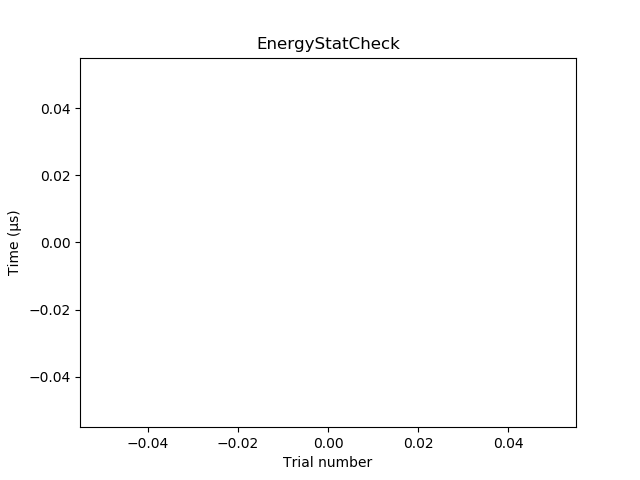
\includegraphics[width=10cm,height=10cm,keepaspectratio]{RuntimeResults_SystemA/CFunctions/EnergyStatCheck_scatter.png}
	\caption{Scatter plot of C-Functions runtime for EnergyStatCheck for SystemA}
	\label{fig:C-Functions|EnergyStatCheck|SystemA}
\end{figure}

\begin{figure}[H]
	\centering
	\includegraphics[width=10cm,height=10cm,keepaspectratio]{RuntimeResults_SystemA/CFunctions/GetSocketNum_scatter.png}
	\caption{Scatter plot of C-Functions runtime for GetSocketNum for SystemA}
	\label{fig:C-Functions|GetSocketNum|SystemA}
\end{figure}

\begin{figure}[H]
	\centering
	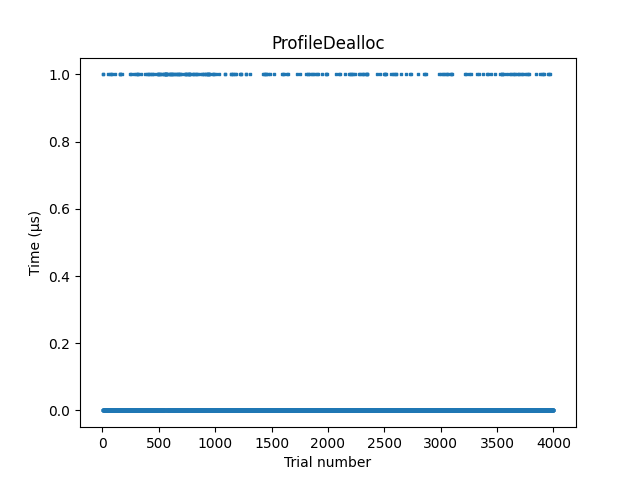
\includegraphics[width=10cm,height=10cm,keepaspectratio]{RuntimeResults_SystemB/CFunctions/ProfileDealloc_scatter.png}
	\caption{Scatter plot of C-Functions runtime for ProfileDealloc for SystemB}
	\label{fig:C-Functions|ProfileDealloc|SystemB}
\end{figure}

\begin{figure}[H]
	\centering
	\includegraphics[width=10cm,height=10cm,keepaspectratio]{RuntimeResults_SystemB/CFunctions/ProfileInit_scatter.png}
	\caption{Scatter plot of C-Functions runtime for ProfileInit for SystemB}
	\label{fig:C-Functions|ProfileInit|SystemB}
\end{figure}

\begin{figure}[H]
	\centering
	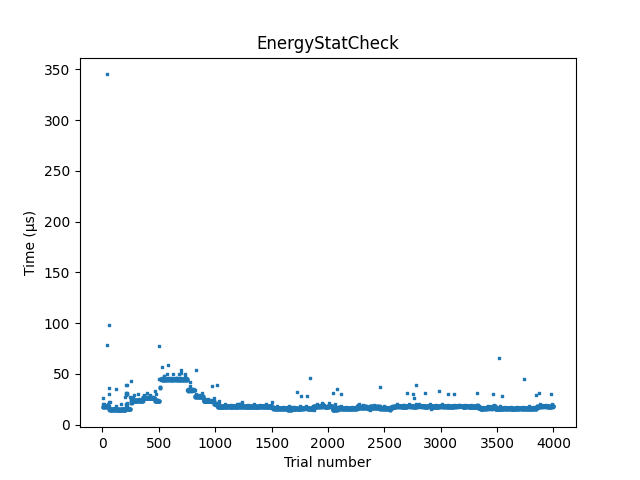
\includegraphics[width=10cm,height=10cm,keepaspectratio]{RuntimeResults_SystemB/CFunctions/EnergyStatCheck_scatter.png}
	\caption{Scatter plot of C-Functions runtime for EnergyStatCheck for SystemB}
	\label{fig:C-Functions|EnergyStatCheck|SystemB}
\end{figure}

\begin{figure}[H]
	\centering
	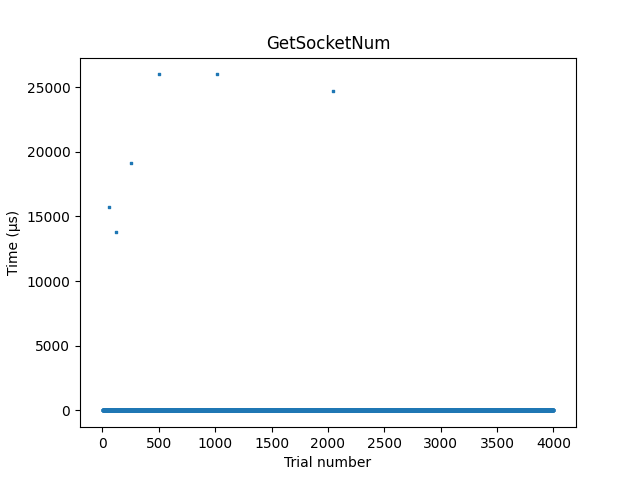
\includegraphics[width=10cm,height=10cm,keepaspectratio]{RuntimeResults_SystemB/CFunctions/GetSocketNum_scatter.png}
	\caption{Scatter plot of C-Functions runtime for GetSocketNum for SystemB}
	\label{fig:C-Functions|GetSocketNum|SystemB}
\end{figure}

\begin{figure}[H]
	\centering
	\includegraphics[width=10cm,height=10cm,keepaspectratio]{RuntimeResults_SystemA/JavaFunctions/ProfileDealloc_scatter.png}
	\caption{Scatter plot of Java-Functions runtime for ProfileDealloc for SystemA}
	\label{fig:Java-Functions|ProfileDealloc|SystemA}
\end{figure}

\begin{figure}[H]
	\centering
	\includegraphics[width=10cm,height=10cm,keepaspectratio]{RuntimeResults_SystemA/JavaFunctions/ProfileInit_scatter.png}
	\caption{Scatter plot of Java-Functions runtime for ProfileInit for SystemA}
	\label{fig:Java-Functions|ProfileInit|SystemA}
\end{figure}

\begin{figure}[H]
	\centering
	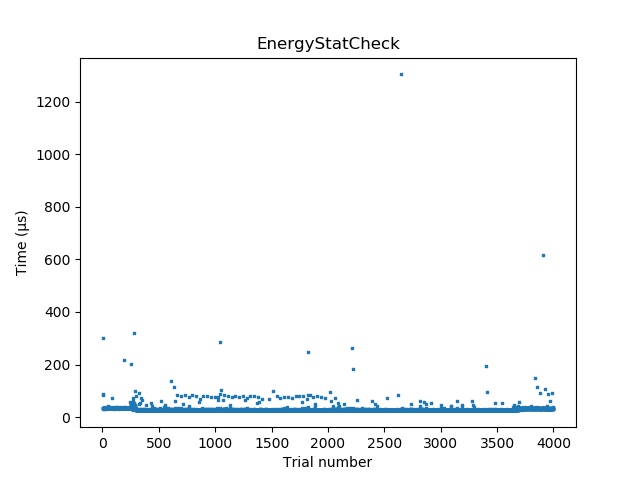
\includegraphics[width=10cm,height=10cm,keepaspectratio]{RuntimeResults_SystemA/JavaFunctions/EnergyStatCheck_scatter.png}
	\caption{Scatter plot of Java-Functions runtime for EnergyStatCheck for SystemA}
	\label{fig:Java-Functions|EnergyStatCheck|SystemA}
\end{figure}

\begin{figure}[H]
	\centering
	\includegraphics[width=10cm,height=10cm,keepaspectratio]{RuntimeResults_SystemA/JavaFunctions/GetSocketNum_scatter.png}
	\caption{Scatter plot of Java-Functions runtime for GetSocketNum for SystemA}
	\label{fig:Java-Functions|GetSocketNum|SystemA}
\end{figure}

\begin{figure}[H]
	\centering
	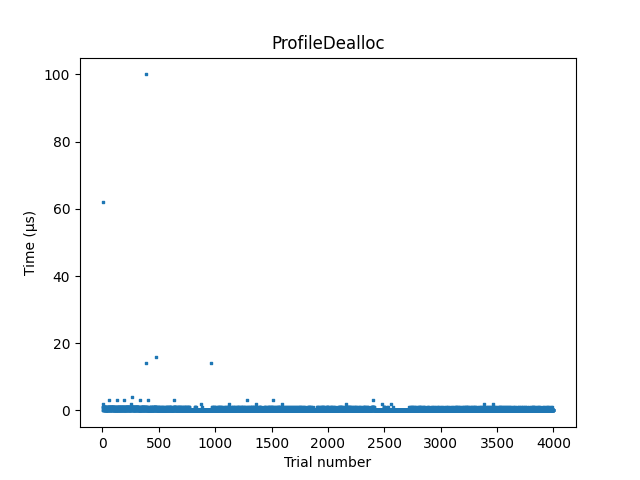
\includegraphics[width=10cm,height=10cm,keepaspectratio]{RuntimeResults_SystemB/JavaFunctions/ProfileDealloc_scatter.png}
	\caption{Scatter plot of Java-Functions runtime for ProfileDealloc for SystemB}
	\label{fig:Java-Functions|ProfileDealloc|SystemB}
\end{figure}

\begin{figure}[H]
	\centering
	\includegraphics[width=10cm,height=10cm,keepaspectratio]{RuntimeResults_SystemB/JavaFunctions/ProfileInit_scatter.png}
	\caption{Scatter plot of Java-Functions runtime for ProfileInit for SystemB}
	\label{fig:Java-Functions|ProfileInit|SystemB}
\end{figure}

\begin{figure}[H]
	\centering
	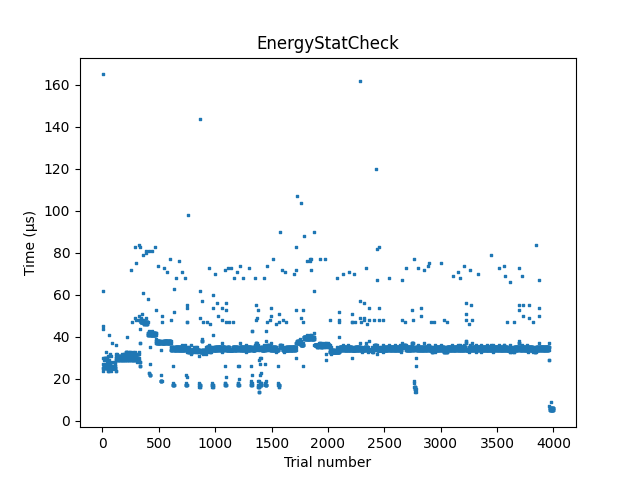
\includegraphics[width=10cm,height=10cm,keepaspectratio]{RuntimeResults_SystemB/JavaFunctions/EnergyStatCheck_scatter.png}
	\caption{Scatter plot of Java-Functions runtime for EnergyStatCheck for SystemB}
	\label{fig:Java-Functions|EnergyStatCheck|SystemB}
\end{figure}

\begin{figure}[H]
	\centering
	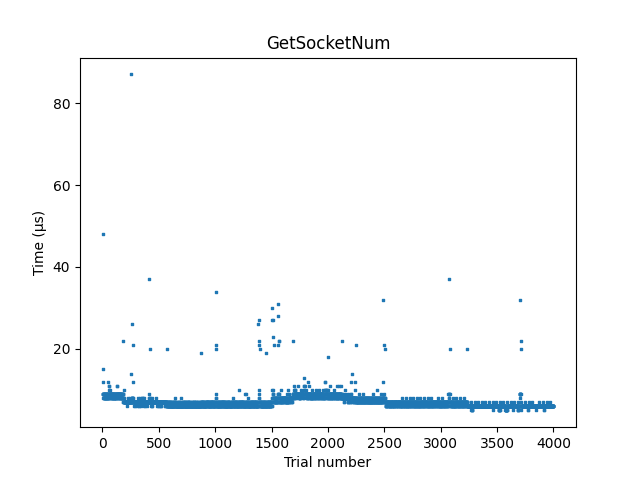
\includegraphics[width=10cm,height=10cm,keepaspectratio]{RuntimeResults_SystemB/JavaFunctions/GetSocketNum_scatter.png}
	\caption{Scatter plot of Java-Functions runtime for GetSocketNum for SystemB}
	\label{fig:Java-Functions|GetSocketNum|SystemB}
\end{figure}

\begin{figure}[H]
	\centering
	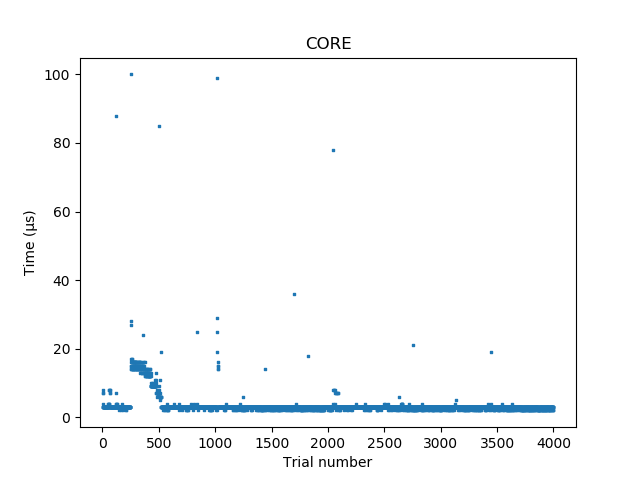
\includegraphics[width=10cm,height=10cm,keepaspectratio]{RuntimeResults_SystemB/PerSocketMSRReadings/Socket0/CORE_scatter.png}
	\caption{Scatter plot of Per-Socket-MSR-Readings runtime for CORE for SystemB}
	\label{fig:Per-Socket-MSR-Readings|CORE|SystemB}
\end{figure}

\begin{figure}[H]
	\centering
	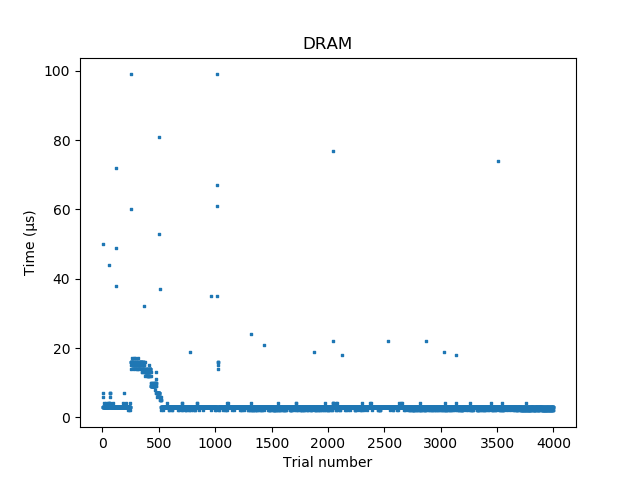
\includegraphics[width=10cm,height=10cm,keepaspectratio]{RuntimeResults_SystemB/PerSocketMSRReadings/Socket0/DRAM_scatter.png}
	\caption{Scatter plot of Per-Socket-MSR-Readings runtime for DRAM for SystemB}
	\label{fig:Per-Socket-MSR-Readings|DRAM|SystemB}
\end{figure}

\begin{figure}[H]
	\centering
	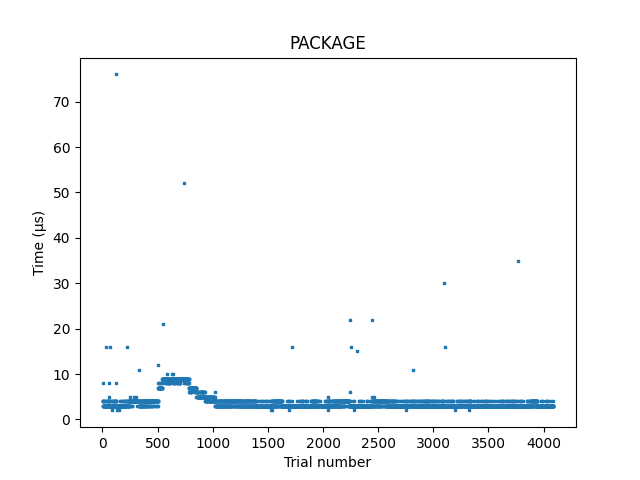
\includegraphics[width=10cm,height=10cm,keepaspectratio]{RuntimeResults_SystemB/PerSocketMSRReadings/Socket0/PACKAGE_scatter.png}
	\caption{Scatter plot of Per-Socket-MSR-Readings runtime for PACKAGE for SystemB}
	\label{fig:Per-Socket-MSR-Readings|PACKAGE|SystemB}
\end{figure}

\begin{figure}[H]
	\centering
	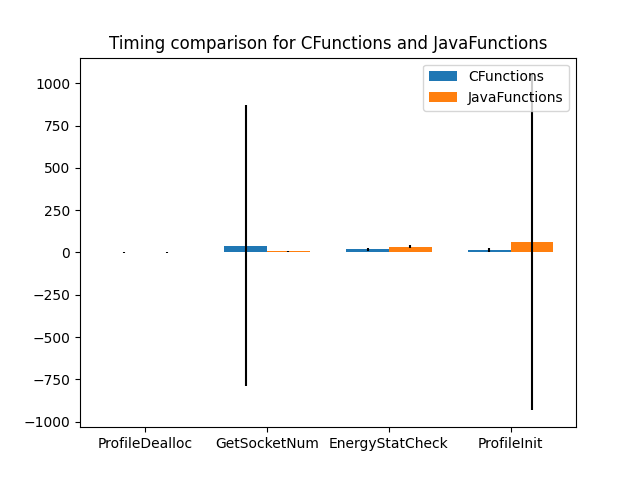
\includegraphics[width=10cm,height=10cm,keepaspectratio]{RuntimeResults_SystemB/CFunctions-JavaFunctions-bar_graph.png}
	\caption{Bar graph comparing Java and C function runtime}
	\label{fig:bar-graph||SystemB}
\end{figure}

\begin{figure}[H]
	\centering
	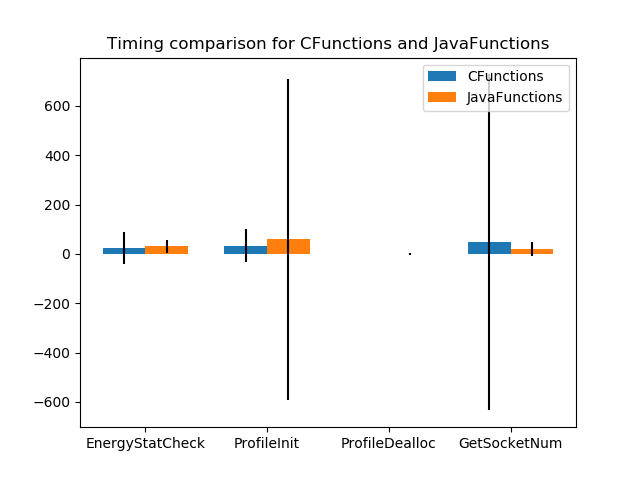
\includegraphics[width=10cm,height=10cm,keepaspectratio]{RuntimeResults_SystemA/CFunctions-JavaFunctions-bar_graph.png}
	\caption{Bar graph comparing Java and C function runtime}
	\label{fig:bar-graph||SystemA}
\end{figure}

